%%%%%%%%%%%%%%%%%%%%%%%%%%%%%%%%%%%%%%%%%
% Szablon pracy dyplomowej
% Wydział Informatyki 
% Zachodniopomorski Uniwersytet Technologiczny w Szczecinie
% autor Joanna Kołodziejczyk (jkolodziejczyk@zut.edu.pl)
% Bardzo wczesnym pierwowzorem szablonu był
% The Legrand Orange Book
% Version 2.1 (26/09/2018)
%
% Modifications to LOB assigned by %JK
%%%%%%%%%%%%%%%%%%%%%%%%%%%%%%%%%%%%%%%%%


%----------------------------------------------------------------------------------------
%	CHAPTER 2
%----------------------------------------------------------------------------------------

\chapter{Opracowany algorytm}
\label{ch:opracowany-algorytm}
\chaptermark{Opracowany algorytm} % Tekst, który wyświetli się w nagłówku strony,  jeżeli jest za długi tytuł rozdziału


\section{Proces uczenia klasyfikatora}
\label{sec:proces-uczenia-klasyfikatora}
Proces uczenia klasyfikatora jest kluczowym etapem budowy modelu uczenia maszynowego.
Jeżeli na tym etapie dojdzie do błędu, będzie to rzutować na działanie całej aplikacji.
Częstym zjawiskiem w uczeniu maszynowym jest przeuczenie (ang. \textit{overfitting}).
Polega ono na wykrywaniu pozornych prawidłowości w dużej ilości danych, gdzie prawdziwe prawidłowości są prostsze lub słabsze, lub są maskowane przez błędy, lub są całkowicie nieistniejące \cite{overfitting}.

TODO - do dokończenia

\subsection{Przygotowanie danych uczących}
\label{subsec:przygotowanie-danych-uczacych}
W rozdziale \ref{ch:preparing_data_set} przedstawiono opracowany zbiór zdjęć z kamery samochodowej zawierający poruszające się pojazdy wraz z ich tablicami rejestracyjnymi.
Klasyfikatory działają jednak w inny sposób niż ludzki mózg i wymagają innych wartości, na których będą mogły podejmować decyzje.
W niniejszej pracy zdecydowano się wykorzystać cechy Haara jako cechy reprezentujące poszukiwane obiekty.
W celu wyuczenia klasyfikatora, należało opracowany wcześniej zbiór przetworzyć, aby każda negatywna i pozytywna próbka miała swoją reprezentację liczbową.
Na rysunku~\ref{fig:haar_feats_dataset_prepare} przedstawiono schemat blokowy procesu przygotowania danych uczących dla klasyfikatora.
\begin{figure}[!ht]
    \centering
    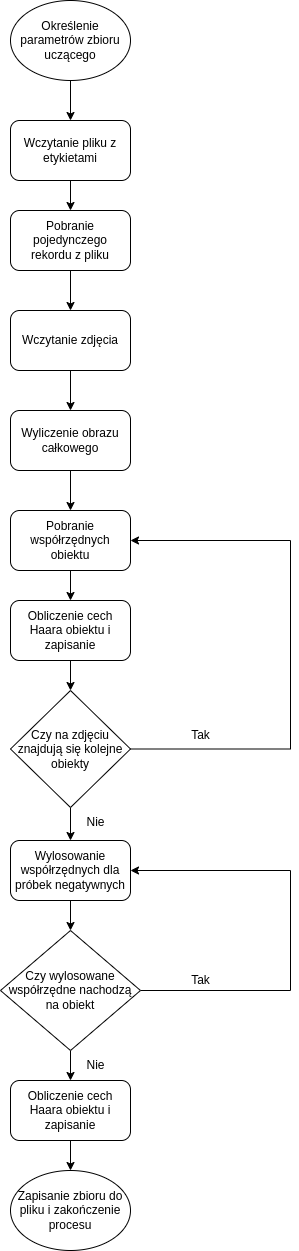
\includegraphics[scale=0.4]{Pictures/prepare_haar_dataset}
    \caption{Schemat blokowy przygotowania danych uczących dla klasyfikatora (źródło: opracowanie własne)}
    \label{fig:haar_feats_dataset_prepare}
\end{figure}
\FloatBarrier
@todo
jakie cechy haara (przedstawienie szablonów), opisać blok, pokazać zdjęcia z uczenia z szablonami

\subsection{Uczenie klasyfikatora}
W niniejszej pracy zaimplementowano i wykorzystano algorytm wzmacniający RealBoost oparty o koszyki (ang. \textit{bins}).
Takie podejście zostało zaprezentowane po raz pierwszy w \cite{1689652}.
Na wejściu metody uczącej funkcja przyjmuje cechy uczące oraz ich etykiety.
Dla każdej cechy obliczane są wartości maksymalne i minimalne.
Ustalane są one poprzez posortowanie wartości konkretnej cechy ze wszystkich próbek ze zbioru uczącego.
Algorytm dodaje odpowiedni margines, aby odrzucić skrajne wyniki.
Współczynnik ten ustalono na poziomie $0.05$.
Oznacza to, że dla zbioru o wielkości 100 próbek, odrzucone zostanie 5 pierwszych i 5 ostatnich wartości cech to wyznaczenia wartości brzegowych.
Następnie przypisywane są indeksy koszyków do poszczególnych cech.
Kolejnym krokiem jest przygotowanie indeksów, które przechowują informację o tym czy cecha dla konkretnego koszyka powiązana jest z próbką pozytywną czy negatywną.
Po przygotowaniu powyższych danych, algorytm przechodzi do wybrania najważniejszych cech z punktu widzenia klasyfikatora.
Obliczane jest to poprzez iterację po wszystkich cechach i określeniu cechy dla każdego klasyfikatora o najmniejszym błędzie.
Wyznaczane jest to za pomocą funkcji logit, która jest wyznaczana dla każdego z koszyków z osobna.
Na koniec dochodzi do reważenia wag.
Czynność jest powtarza dla każdego słabego klasyfikatora.
Algorytm \ref{lst:fit_realboostbins} ukazuje fragment metody uczącej odpowiedzialny za wyliczenie odpowiedzi dla każdego ze słabych klasyfikatorów i wyznaczenie indeksów najlepszych cech.
\begin{lstlisting}[language=Python, caption=Procedura ucząca klasyfikator RealBoostBins, label={lst:fit_realboostbins}]
w = np.ones(m) / m
for t in range(self.T_):
    j_best = None
    logits_best = None
    err_exp_best = np.inf
    for j in range(n):
        logits = np.zeros(self.B_)
        for b in range(self.B_):
            W_positive = w[indexer_positive[j, b]].sum()
            W_negative = w[indexer_negative[j, b]].sum()
            logits[b] = self.logit(W_positive, W_negative)
        err_exp = np.sum(w * np.exp(-yy * logits[X_binned[:, j]]))
        if err_exp < err_exp_best:
            err_exp_best = err_exp
            logits_best = logits
            j_best = j
    self.feature_indexes_[t] = j_best
    self.logits_[t] = logits_best
    w = w * np.exp(-yy * logits_best[X_binned[:, j_best]])
    w /= err_exp_best

\end{lstlisting}
Na rysunku \ref{fig:fit_realboostbins} przedstawiono schemat blokowy uczenia klasyfikatora.
\begin{figure}[!ht]
    \centering
    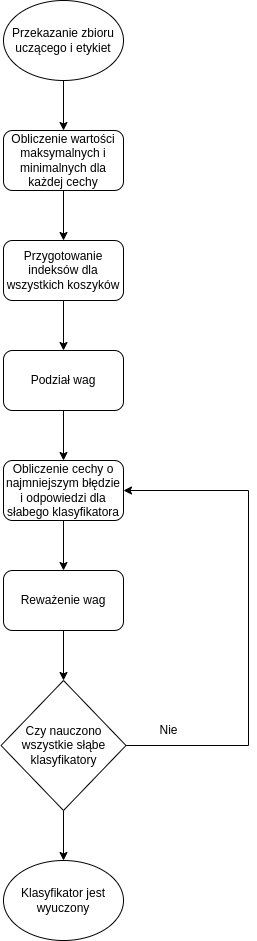
\includegraphics[scale=0.4]{Pictures/fit_realboostbins}
    \caption{Schemat blokowy funkcji uczącej klasyfikatora RealBoostBins (źródło: opracowanie własne)}
    \label{fig:fit_realboostbins}
\end{figure}
\FloatBarrier


\section{Schemat algorytmu}
@todo
diagram graficzny

\subsection{Algorytm detekcji}
@todo

\subsection{Algorytm segmentacji i rozpoznawania znaków}
@todo


\section{Biblioteki użyte w programie}
Środowisko Python jest niezwykle popularne m.in. ze względu na mnogość dostępnych gotowych bilbiotek.
Jednym z celów pracy było zaimplementowanie algorytmu uczącego i klasyfikującego.
Cel ten udało się zrealizować, natomiast nie byłoby to możliwe bez użycia gotowych rozwiązań do elementarnych operacji t.j. listowanie plików w katalogach, odczyt i zapis zdjęć, pobieranie pojedynczych klatek z filmu wideo czy operacje na tablicach.
Poniżej wymieniono i opisano najważniejsze oraz najczęściej używane biblioteki w opisywanej pracy.

\subsection{OpenCV}
OpenCV jest biblioteką o otwartym źródle (ang. \textit{open source}) \cite{open_cv,open_cv_docs} .
Do jej głównych zastosowań należą przetwarzanie obrazów oraz uczenie maszynowe.
W przedstawionym programie wykorzystano najnowszą dostępną wersję na moment pisania pracy $4.6.0$.
Została zaprojektowana, aby zapewnić ustandaryzowaną infrastrukturę dla aplikacji widzenia komputerowego.
Oprogramowanie dystrybuowane jest na licencji BSD.
Pierwsza wersja została opracowana w roku 1999.
Oryginalnie powstała w języku C++, natomiast istnieją biblioteki pozwalające używać jej w innych językach programowania.
Bibliotekę można podzielić na kilka głównych modułów:
\begin{itemize}
    \item Przetwarzanie obrazów - moduł zawiera zestaw metod do przeprowadzania takich operacji jak filtrowanie, przekształcenia geometryczne, zmiana przestrzeni kolorów, histogramy
    \item Przetwarzanie wideo - zestaw metod, które pozwalają na m. in. usuwanie tła, śledzenie obiektów, wykrywanie ruchu
    \item Operacje wejścia/wyjścia na wideo - wyciąganie poszczególnych klatek z wideo, kodowanie, zapis i odczyt wideo
    \item HighGUI - moduł służący do wizualizacji wyników, wyświetlania okien, zaznaczania ROI (ang. \textit{Region of interest})
\end{itemize}

Poniżej wymieniono użyte w stworzonym programie funkcje wraz z krótkim opisem ich zastosowania:
\begin{itemize}
    \item \textit{videoCapture} - przechwytywanie obrazów z pliku wideo
    \item \textit{cvtColor} - zmiana przestrzeni barw w obrazie
    \item \textit{imread} - wczytanie obrazu z pliku
    \item \textit{imshow} - wyświetlenie obrazu
    \item \textit{imwrite} - zapis obrazu do pliku
    \item \textit{rectangle} - rysowanie prostokąta na obrazie
    \item \textit{putText} - umiejscowienie tekstu na obrazie
    \item \textit{addWeighted} - połączenie dwóch obrazów poprzez nałożenie ich na siebie
    \item \textit{thresholding} - binaryzacja obrazu
    \item \textit{GaussianBlur} - wygładzanie obrazu za pomocą funkcji Gaussa
    \item \textit{Canny} - wykrywanie krawędzi za pomocą algorytmu Johna F. Canny'ego \cite{4767851}
    \item \textit{findContours} - wykrywanie konturów obiektów (punktów o tym samym kolorze lub intensywności łączących się w krzywe)
    \item \textit{resize} - zmiana wielkości obrazu
    \item \textit{imdecode} - odczytywanie zdjęcia z bufora
\end{itemize}

\subsection{Tesseract OCR}
Biblioteka Tesseract jest pakietem składającym się z programu lini poleceń \textit{tesseract} oraz silnika OCR \textit{libtesseract} \cite{tesseract}.
Tesseract powstał między rokiem 1985, a 1994 na potrzeby firmy Hewlett-Packard.
W roku 2005 firma upubliczniła bibliotekę jako rozwiązanie \textit{open-source}.
Od początku 2006 do listopada 2018 za rozwój Tesseract odpowiedzialna była firma Google.
Obecnie głównym programistą projektu jest Ray Smith.
Silnik programu oparty jest o język programowania C++.
W celu wykorzystania jej w opisywanym programie, użyto nakładki \textit{pytesseract} \cite{pytesseract}.
Autorzy deklarują, że najnowsza wersja 5, wydana w listopadzie 2021, wspiera ponad 100 języków.
Biblioteka wykorzystuje rekurencyjne sieci neuronowe LSTM (ang. \textit{Long Short-Temp Memory}) \cite{lstm}.

\subsection{Numpy}

\subsection{Sklearn}

\subsection{Pickle}

\subsection{Numba}
Biblioteka od przyspieszania kodu (jit)